% (C) Marc Lijour, 2017 
% Licensed under a Creative Commons License BY-SA
% https://creativecommons.org/licenses/by-sa/2.5/ca/
% Presentation for Mexican High School Students studying in Toronto 
% authored by Marc Lijour, July 2017
% 
% ======================================================================================================
%                                     Technology: past, present and future
% ======================================================================================================
\section{Technology: Past, Present, and Future}
\frame{
	\frametitle{Economics of Technology}
	\begin{figure}
	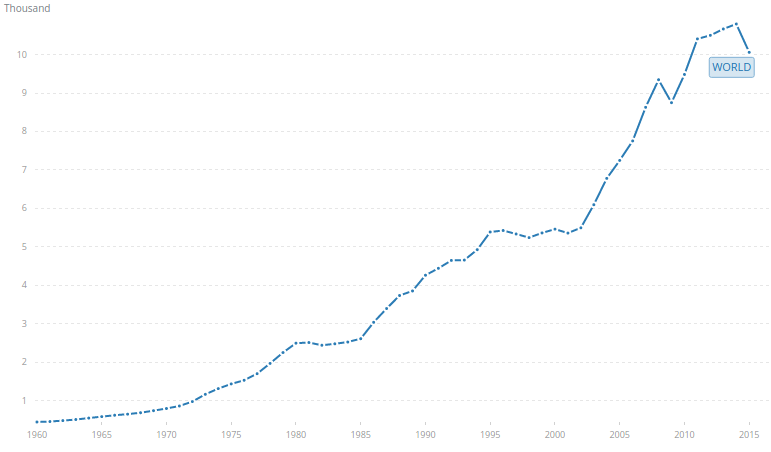
\includegraphics[height=6cm]{../pics/worldbank-GDP-per-capita-1960-2015}
	\caption{World GDP per capita, Credit: \href{http://data.worldbank.org/indicator/NY.GDP.PCAP.CD?end=2015&start=1960}{World Bank, 2017}}
	\end{figure}
}

\frame{
	\frametitle{Emerging Technologies  (\href{http://www.gartner.com/technology/research/hype-cycles/}{Gartner's Hype Cycle}, 2015)}
	\begin{figure}
	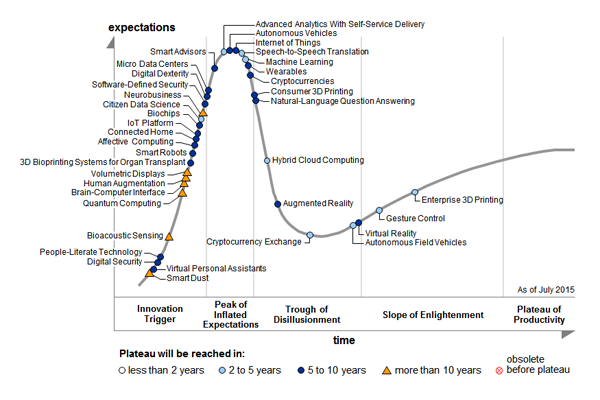
\includegraphics[width=11cm]{../pics/gartner2015_emerging-tech-hc}
	\end{figure}
}

\begin{frame}
	\frametitle{The 4$^{th}$ Industrial Revolution}
	\framesubtitle{Everyone talks about it -Businesses \& Government alike}
	\begin{figure}
		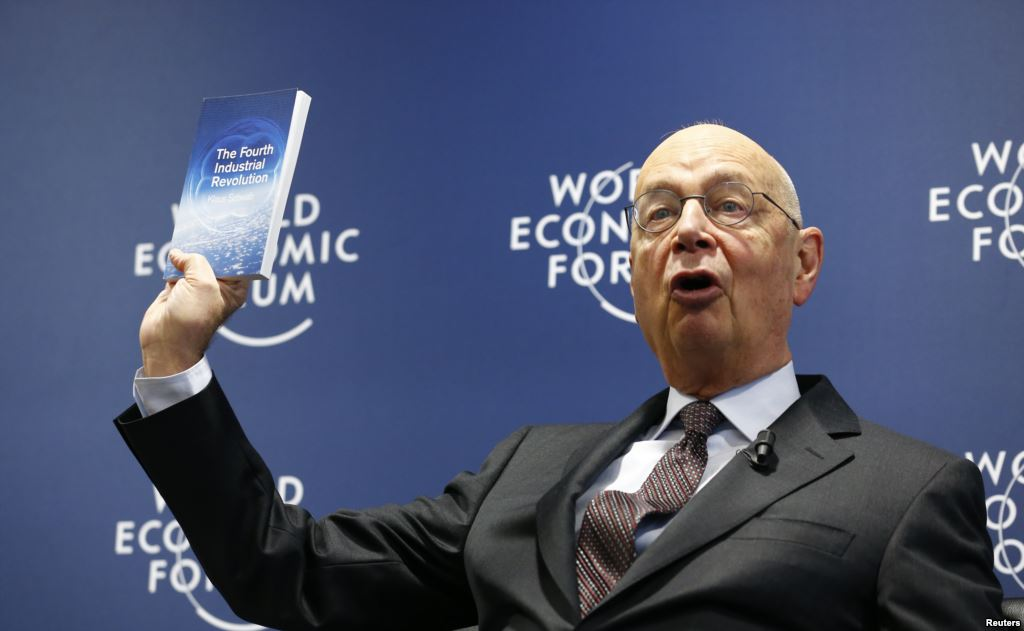
\includegraphics[width=11cm]{../../pics/Schwab-4th-revolution-book-cover}
		\caption{The topic of conversation since Davos~2016 (Credit: \href{http://www.voanews.com/a/wef-founder-world-unprepared-to-deal-with-fourth-industrial-revolution/3143406.html}{Reuters})}
	\end{figure}
\end{frame}

\frame{
	\frametitle{The 4$^{th}$ Industrial Revolution}
	\framesubtitle{}
	\begin{block}{}
%		\begin{quote}
		``The new technology revolution, which entails nothing less than a transformation of mankind.'' ---Klaus Schwab, founder and executive chairman of the World Economic Forum
%		\end{quote}
	\end{block}
	\vspace{2cm}
	\fullcite{schwab2016}
}

% ======================================================================================================
%                                     Technology areas
% ======================================================================================================
\section{Booming Areas}
\subsection{Internet of Things}
\frame{
	\frametitle{The IoT market value at stake}
	\framesubtitle{\$19T over 10 years according to Cisco}
	\begin{figure}
	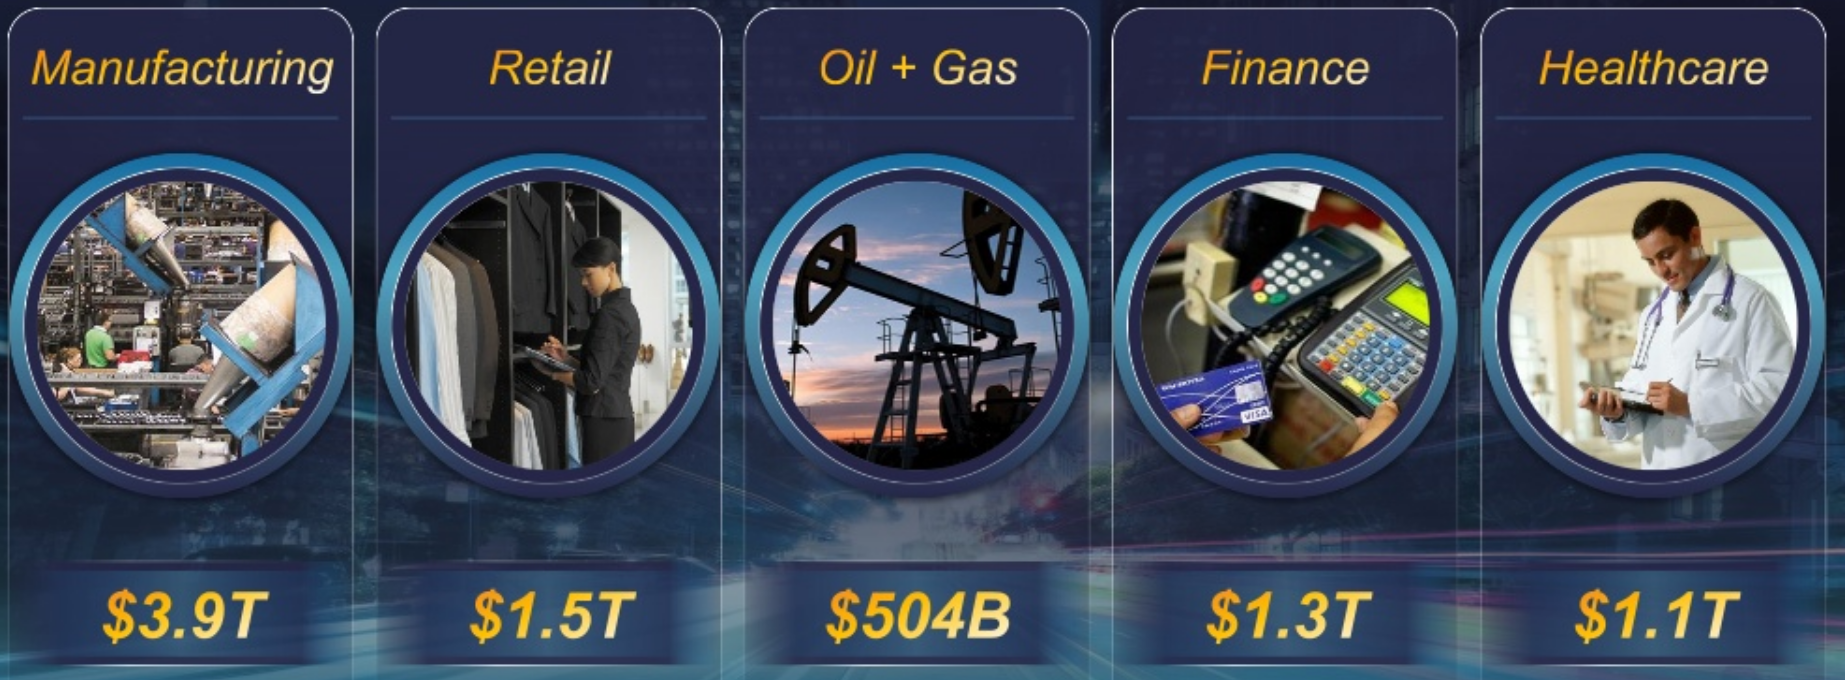
\includegraphics[width=11cm]{../../pics/Cisco-IoE-main-verticals}
	\caption{Verticals with highest \$ potential Credit: \href{http://www.slideshare.net/Cisco/john-chambers-cisco-live-keynote-presentation}{John Chambers Keynote (Cisco, 2014)}}
	\end{figure}
}

\subsection{Artificial Intelligence}
\frame{
	\frametitle{Artificial Intelligence}
	\begin{figure}
	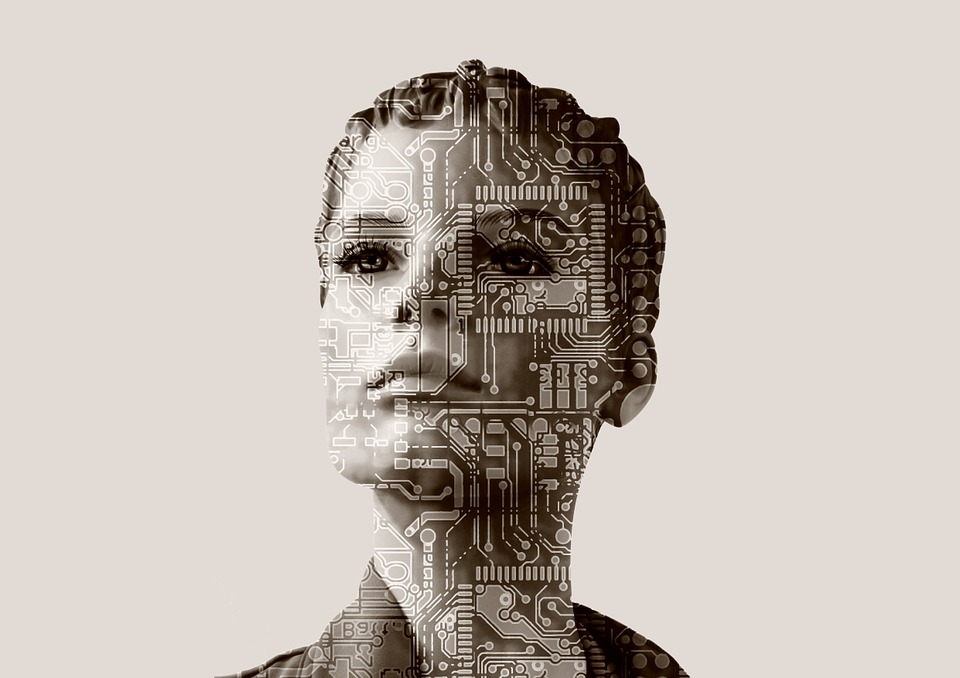
\includegraphics[width=10cm]{../../pics/ai_woman-506322_960_720}
	\caption{Credit: \href{https://pixabay.com/en/woman-artificial-intelligence-506322/}{geralt}}
	\end{figure}
}

\subsection{Blockchain}
\frame{
	\frametitle{Blockchain}
	\begin{figure}
	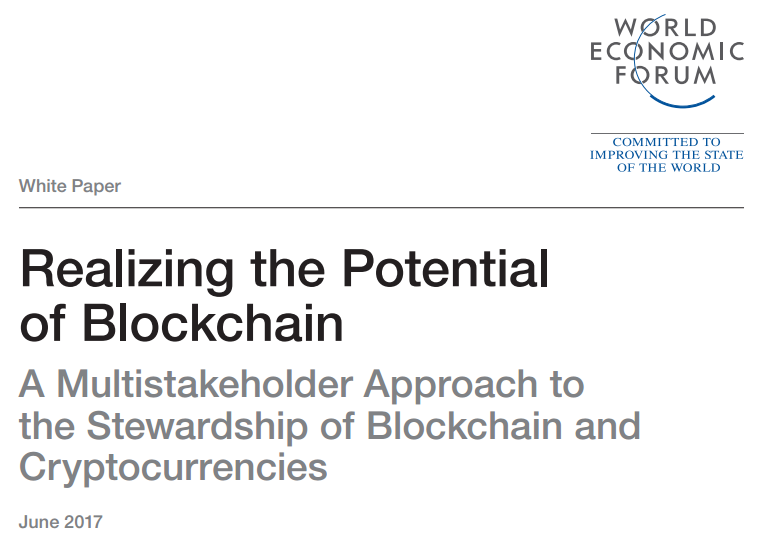
\includegraphics[width=10cm]{../../pics/wef2017-whitepaper-cover}
	\caption{Credit: \href{http://www3.weforum.org/docs/WEF_Realizing_Potential_Blockchain.pdf}{World Economic Forum}}
	\end{figure}
}
\frame{
	\frametitle{Case Study: ColliderX}
	\framesubtitle{\url{https://www.collider-x.org}}
	\begin{itemize}
		\item World-first Open Source Crowdfunded R\&D Hub focusing on Blockchain and related technologies (AI, IoT, ...)
		\pause
		\item Building \href{http://www3.weforum.org/docs/WEF_Realizing_Potential_Blockchain.pdf}{the digital infrastructure of tomorrow}
		\pause
		\item Now building a Blockchain \href{https://www.ic.gc.ca/eic/site/093.nsf/eng/00003.html}{Innovation Supercluster} in Canada
		\pause
		\item Open to all researchers/tinkerers and backers in the world
	\end{itemize}
}

% ======================================================================================================
%                                     Career Implications
% ======================================================================================================
\section{Career Implications}

\frame{
	\frametitle{Career Implications}
	\begin{itemize}
		\item Newer \& better jobs (old jobs go away, new jobs appear)
		\pause
		\item \href{https://www.ictc-ctic.ca/the-next-talent-wave-navigating-the-digital-shift-ictcs-labour-market-outlook-report-2017-2021/}{216,000 new ICT jobs in Canada} in the next 3 years
		\pause
		\item Life-long Learning
		\pause
		\item Entrepreneuring (start-ups, contract work / self-branding, intrapreneurship...)
	\end{itemize}
}

\frame{
	\frametitle{A new role for Digitization Leaders}
	\begin{figure}
	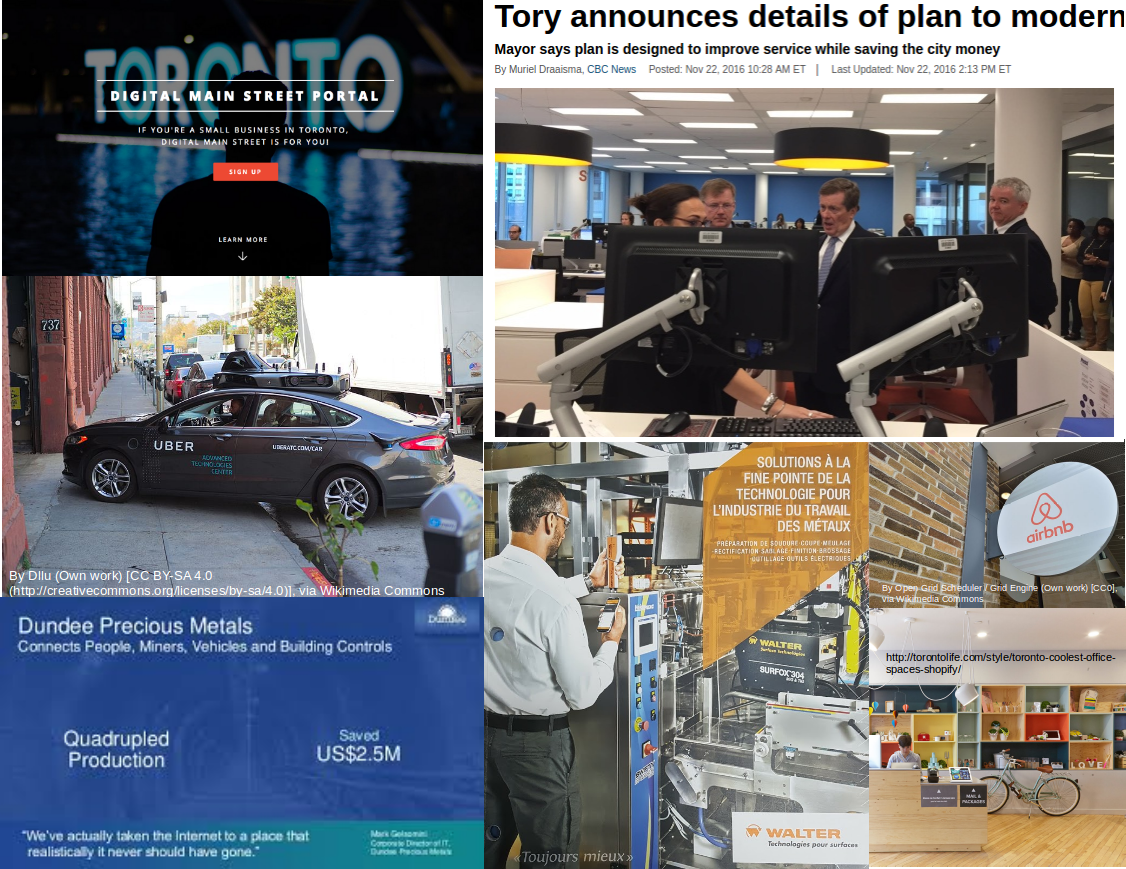
\includegraphics[width=10cm]{../pics/patchwork-digitization-in-Toronto}
	\end{figure}
}

\begin{frame}
	\frametitle{Open Source runs (almost) Everything}
	\framesubtitle{2015 was an inflexion point}
	\begin{figure} % extracts from articles and other sources published on the Web
		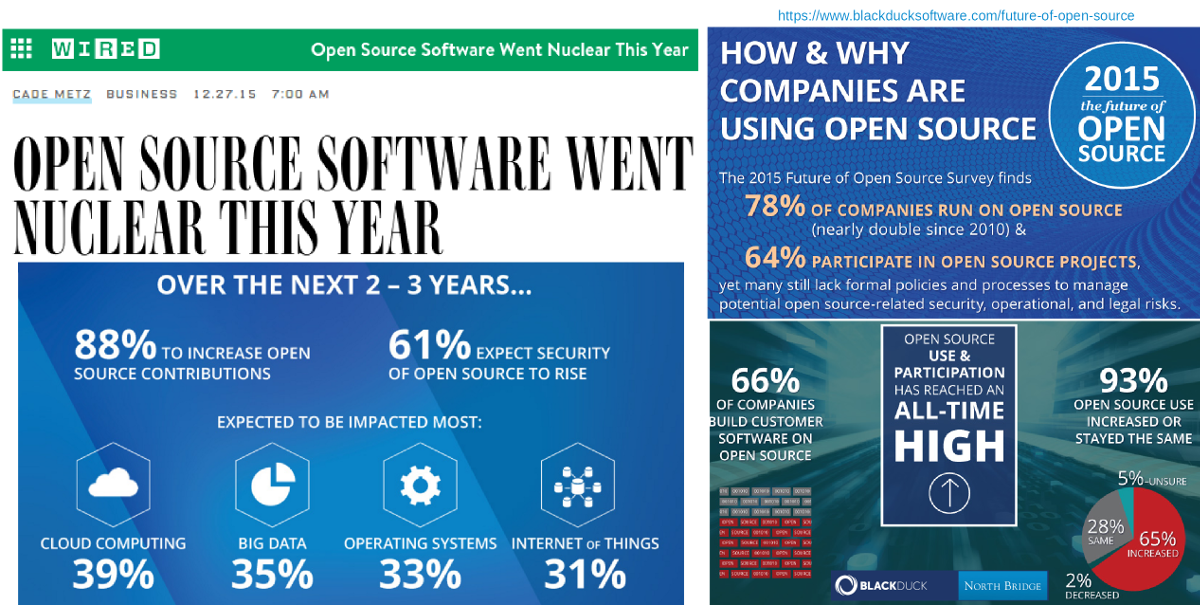
\includegraphics[width=11cm]{../pics/pic-open-source-went-nuclear-non-interlaced}
	\end{figure}
\end{frame}

\frame{
	\frametitle{Formation of Tech Clusters}
	\framesubtitle{e.g. Opportunities in Ontario}
	\begin{columns}
	\column{0.5\textwidth}
		\begin{figure}
		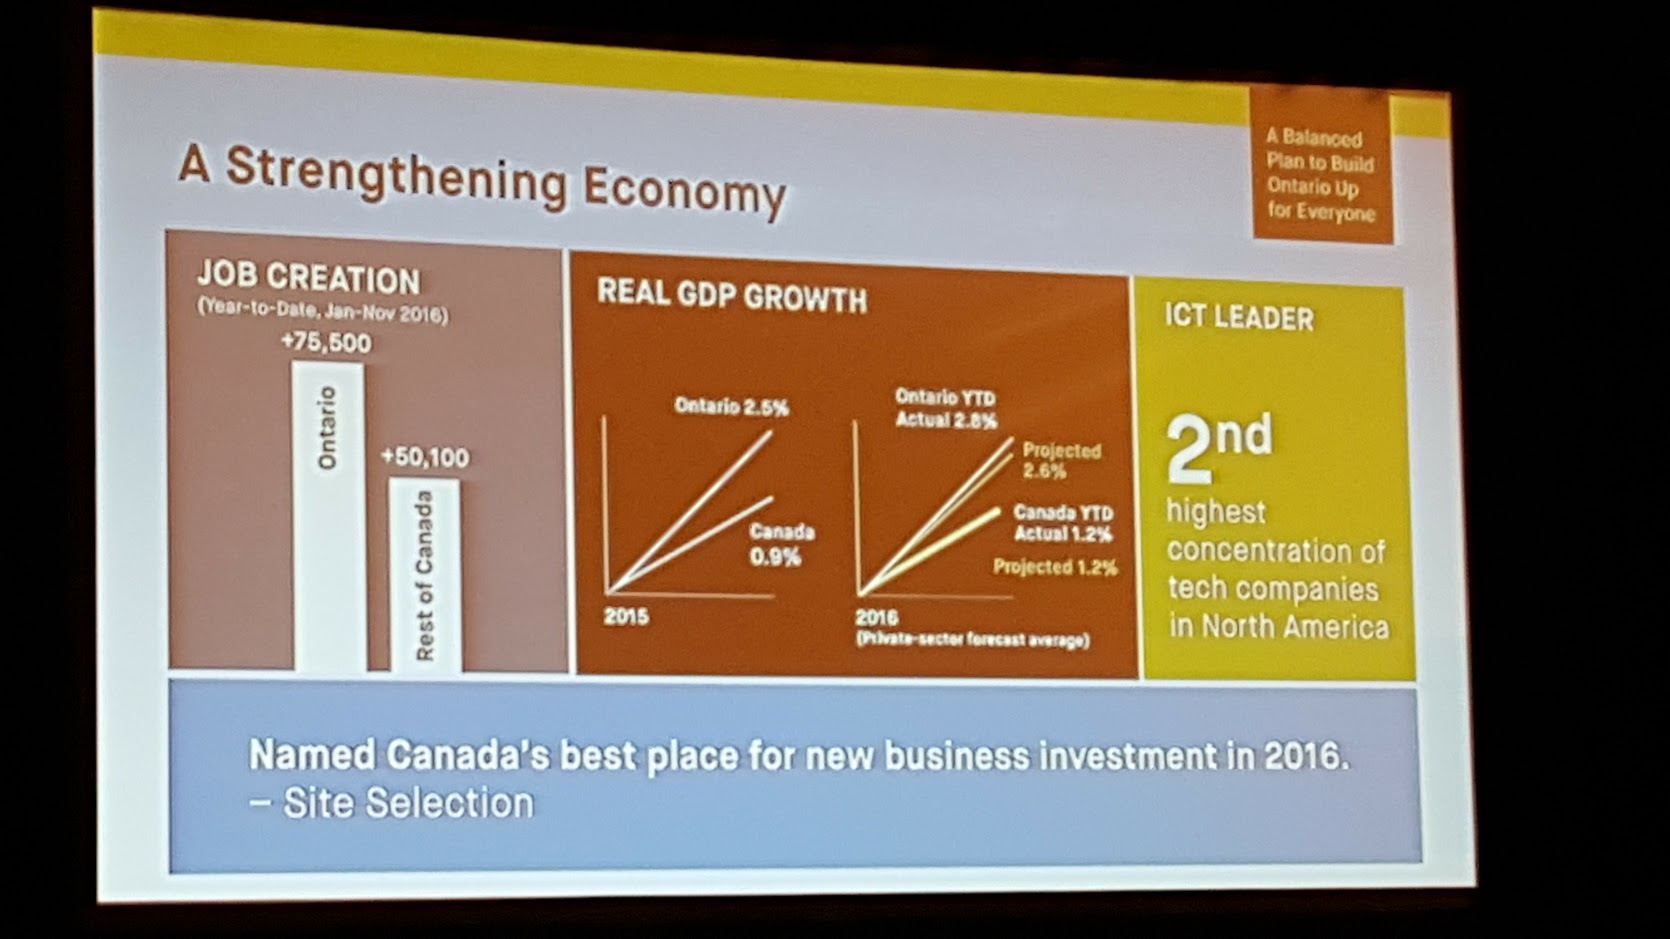
\includegraphics[width=7cm]{../pics/Wynne-economy-2016}
		\end{figure}
	\column{0.5\textwidth}
		\begin{figure}
		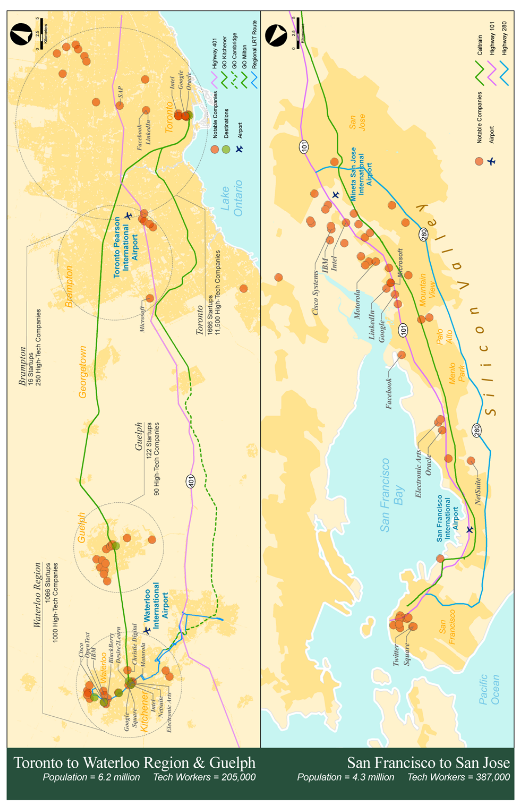
\includegraphics[width=3cm]{../pics/Toronto-Waterloo-corridor}
		\end{figure}
	\end{columns}
}


